
\chapter{动态推荐系统设计}
  \section{前言}
  推荐系统的形式化定义如下:设C是所有用户的集合,S是所有可以推荐给用户的主题的集合。实际上,C和S集合的规模通常很大,如上百万的顾客以及上万款手机主题。设效用函数u()可以计算主题s对用户c的推荐度(如提供商的可靠性(vendor reliability)和产品的可得性(product availability),即$u=C\times S \rightarrow R$,R是一定范围内的全序的非负实数,推荐要研究的问题就是找到推荐度R最大的那些主题S*,如\autoref{equ:fromal}
    \begin{equation}
    \forall c \in C,S^{*}=arg  max_{s \in S} u(c,s)
    \label{equ:fromal}
    \end{equation}
  除了推荐系统自身如冷启动、数据的稀疏性等问题,还有一个关注点就是推荐系统的时间效应问题。比较常见的时间效应问题主要反映在用户兴趣的变化、物品流行度的变化以及手机主题的季节效应,这些问题都可以利用用户画像解决。本章节主要介绍如何搭建一个具有长尾性、实时性的动态推荐系统。动态推荐形态由以下几个模块组成:用户画像模型,用户兴趣探索模块,推荐主题模块,推荐算法模块。通用的推荐系统模型流程是:首先,推荐系统把用户画像模型中兴趣需求信息和推荐主题模型中的特征信息匹配,然后使用相应的推荐算法进行计算筛选,找到用户可能感兴趣的推荐主题,最后推荐给用户。

  用户画像模块对应着用户长期兴趣,用户兴趣探索对应着用户短期动态兴趣。短期兴趣的特点是临时、易变;长期兴趣的特点是长久、稳定;用户的短期兴趣可能会转化为长期兴趣,所以需要在推荐时综合考虑长期兴趣和短期兴趣。考虑到推荐系统的时间效应问题,将输入数据集归结为一个四元组,即{用户,物品,行为,时间},通过研究用户的历史行为来预测用户将来的行为。需要解决以下俩个问题:动态评分预测、时效性的影响。首先,动态评分预测问题。数据集可以选用比较直观的显性反馈数据集,即(用户,物品,评分,时间),研究是这样一个问题,给定用户u,物品i,时间t,预测用户u在时间t对物品i的评分r。对于该类问题,与时间无关的评分预测问题算法主要有以下几种:用户兴趣的变化,如年龄增长,从儿童长成青少年壮年;生活状态的变化,由以前的小学生到大学生;社会事件的影响如俩会等。此外还有季节效应问题,一些在春季很流行的,在夏季节未必就很流行。该问题的解决有待进一步思考。对于时效性的影响,每个在线系统都是一个动态系统,但它们有不同的演化速率。比如说,新闻更新很快,但音乐,电影的系统演化的却比较慢。

  本章首先介绍用户画像和兴趣探索模块,其中兴趣探索模块需要根据业务的演化速率来调整迭代深度。然后介绍推荐主题模块,之后介绍推荐算法模块和指标体系,最后做总结。
  
  \section{用户画像和兴趣探索模块}
  目前基于用户画像的推荐,主要用在基于内容的推荐,从最近的RecSys大会(ACM Recommender Systems)上来看,不少公司和研究者也在尝试基于用户画像做Context-Aware的推荐(情境感知,又称上下文感知)。利用用户的画像,结合时间、天气等上下文信息,给用户做一些更加精准化的推荐是一个不错的方向。一个好的推荐系统要给用户提供个性化的、高效的、动态准确的推荐,那么推荐系统应能够获取反映用户多方面的、动态变化的兴趣偏好,推荐系统有必要为用户建立一个用户兴趣探索模型,该模型能获取、表示、存储和修改用户兴趣偏好,能进行推理,对用户进行分类和识别,帮助系统更好地理解用户特征和类别。推荐系统根据用户画像进行推荐,所以用户画像对推荐系统的质量有至关重要的影响。建立用户画像模型之前需要考虑问题有:模型的输入数据有哪些,如何获取模型的输入数据;如何考虑用户的兴趣及需求的变化;建模的对象是谁以及如何建模;模型的输出是什么。用户画像模型的输入数据主构成包括:
  \begin{itemize}
  \item 用户属性,分为社会属性和自然属性,包括用户最基本的如用户的姓名、年龄、职业、收入、学历等信息。用户注册时的对自然属性和社会属性进行初始建模。 
  \item 用户手工输入的信息:是用户主动输出给系统的信息,包括用户在搜索引擎中打出的关键词,用户评论中发布的感兴趣的主题、频道。还有一类重要的信息就是用户反馈的信息,包括用户自己对推荐结果的满意程度;用户标注的浏览页面的感兴趣、不感兴趣或感兴趣的程度等。
  \item 用户的浏览行为和浏览内容:用户浏览的行为和内容体现了用户的兴趣和需求,它们包括浏览次数、频率、停留时间等,浏览页面时的操作(收藏、保存、复制等)、浏览时用户表情的变化等。服务器端保存的日志记录了用户的浏览行为和内容。
  \end{itemize}

  \subsection{用户行为的权重排序}
  用户显式行为数据记录了用户在平台上不同的环节的各种行为,这些行为一方面用于候选集触发算法中的离线计算(主要是点击、浏览),另外一方面,这些行为代表的用户兴趣强弱不同,因此在训练重排序模型时针对不同的行为设定了不同的权重值,以更细地刻画用户的行为强弱程度。此外,用户的购买、试用等行为还作为重排序模型的交叉验证特征值,用于模型的离线训练和在线预测。负反馈数据反映了当前的结果可能在某些方面不能满足用户的需求,因此在后续的候选集触发过程中需要考虑对特定的因素进行过滤或者降权,提高用户体验;同时在重排序的模型训练中,A/B测试结果作为负例参与模型训练。用户画像是刻画用户属性的元数据,其中有些是直接获取的基础数据,有些是经过挖掘的二次数据,这些属性一方面可以用于候选集触发过程中对标签进行加权或降权,另外一方面可以作为重排序模型中的用户维度特征。通过对数据的挖掘可以提取出一些关键词,然后使用这些关键词给主题打标签,用于主题的个性化展示。

  \subsection{用户行为的获取方式}
  对于用户的一些人口属性信息采用了显式方式直接获取,对于用户一些明显的兴趣偏好采用了隐式获取,对于用户潜在的兴趣偏好则通过关联技术启发式获取。显式获取用户兴趣偏好的方法是简单而直接的做法,能准确地反映用户的需求,同时所得的信息比较具体、全面、客观,结果比较可靠。缺点就是数量稀少,原因用户不太愿意花时间来向商家表达自己的喜好,并且这种方法灵活性差,答案存在异质性,当用户兴趣改变时需要用户手动更改系统中用户兴趣。同时该方法对用户不是很人性化。隐式获取法是指系统通过记录用户行为数据,通过权重排序获取用户的兴趣偏好,用户的很多动作都能暗示用户的喜好,包括查询、浏览页面和文章、标记书签、反馈信息、滑屏等。隐式的跟踪可以在建立用户画像基本数据的同时不打扰用户的正常消费活动。这种方法的缺点就是跟踪的结果未必能正确反映用户的兴趣偏好。上述获取兴趣偏好的方法有时受用户教育背景、职业和习惯等因素的限制,用户有时意识不到自己的兴趣主题,因此能为用户提供启发式信息,如领域术语抽取和相似度物品聚类,可以实现领域知识的复用,为用户间的协同提供支持,提高用户兴趣获取质量。用户的兴趣和需求会随着时间和情景发生变化,用户画像模块要考虑到用户长期兴趣偏好和短期兴趣偏好,还要考虑兴趣的变化。因此结合用户画像和用户兴趣探索的动态建模将是团队下一个研究方向,如\autoref{pic:hl_iterate}所示。
  \begin{figure}
    \centering
      \framebox{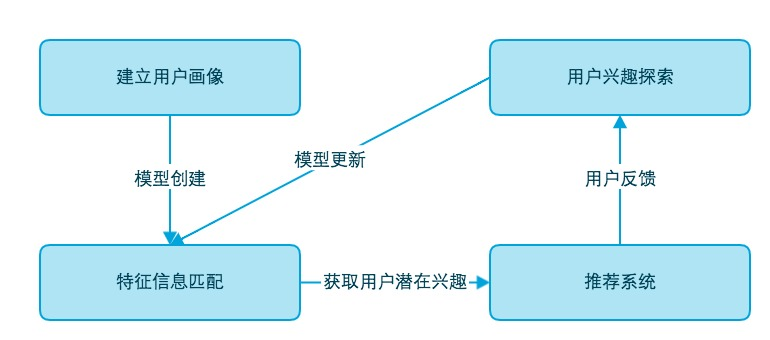
\includegraphics[scale=0.4]{figures/hl_iterate}}
      \figcaption{用户画像的使用}
      \label{pic:hl_iterate}
  \end{figure}

  当前开发阶段的用户画像更新采用了时间窗方法和遗忘机制来反映用户兴趣的变化。更新机制是天级别,所以无法及时跟踪用户兴趣的变化并给出推荐结果,just-in-time型有更强学习效率和动态变化适应能力的建模也是未来的重要研究方向。 

  \section{推荐主题模块}
  推荐主题采用了单用户建模和群组建模,单用户建模针对个体用户进行建模,群组建模是针对一类用户进行建模。动态推荐系统对Top 20\%的活跃用户采用了单用户建模,这样做的的目的有俩个:1,活跃用户的用户行为数据相比较其他用户更多,不存在数据稀疏性问题;2,活跃用户往往消费金额多,单独对其建模有助于提供高质量的推荐服务,有利于提升手机主题转化率。于此同时对剩余用户采用群组建模,这是因为只有对不活跃用户聚类后才可以得到足够多用来建模的数据。

  和用户画像一样,对手机主题进行描述之前要考虑:提取手机主题的什么特征,如何提取,提取的特征用于什么目的,主题的特征描述和用户画像之间有关联。提取到的每个主题特征标签对推荐结果会有什么影响。主题的特征描述向量空间能否自动更新。
  推荐主题的向量空间中的主题特征和用户画像中的兴趣标签进行推荐计算,获得推荐主题的推荐权重,所以推荐主题的向量空间与用户画像密切相关,所有要用同样的标签集来表达用户的兴趣偏好和推荐主题。推荐系统推荐主题包括众多的领域,比如体育、动漫、科技还有诸如音乐、电影等。不同的主题,特征也不相同,动态推荐系统主要采用了基于内容的方法和基于分类的方法两大类方法。 基于内容的方法是从主题本身抽取相关信息来表示主题,具体方法是用加权关键词矢量,该方法通过对标注主题的标签进行统计分析得出的特征向量,通过计算每个标签的信息增量(Information gain),即计算每个特征在主题中出现前后的信息熵之差。在完成主题特征提取后,还需要计算每个特征的权值,权值大的对推荐结果的影响就大。基于分类的方法是把推荐主题放入不同类别中,这样可以把同类主题推荐给对该类主题感兴趣的用户了。文本分类的方法使用了k最近邻方法(KNN)。 主题的类型一部分由第三方设计师自己预先定义,同时利用聚类算法自动产生一些类型。实验表明聚类的精度非常依赖于主题的数量,而且由自动聚类产生的类型可能对用户来说是毫无意义的,因此可以有选择的进行手工选定的类型来分类主题,在没有对应的候选类型或需要进一步划分某类型时,才使用聚类产生的类型。推荐系统推荐给用户的主题首先不能与用户购买过的主题重复,其次也不能与用户刚刚看过的主题不是太形似或者太不相关,这就是所谓的模型过拟合问题(可扩展性问题)。出现这一问题的本质上来自数据的不完备性,解决的主要的方法是引入随机性,使算法收敛到全局最优或者逼近全局最优。针对这一问题考察了被推荐的主题的相关性和冗余性,要同时保证推荐的多样性,又不能与用户看过的主题重复或毫不相关。推荐系统中出现新的主题时,推荐系统尤其是协同过滤系统中,新主题出现后必须等待一段时间才会有用户浏览和评价,而在此之前推荐系统是无法对此主题进行推荐,这就是推荐系统研究的另一个难点和重点——冷启动问题。
  
  \section{推荐算法模块}
  现有的推荐算法类型很多,但是各有各的局限,因此动态推荐系统采用了组合推荐算法,即融合了协同过滤推荐,基于内容推荐和基于关联规则推荐组合推荐算法,他们的主要优缺点对比如所示。
  \begin{table}[htp]
  \centering
  \tabcaption{推荐系统主要算法比较}
  \label{tab:algarithm}
  \begin{tabular}{ |c|p{6cm}|p{6cm}| } \hline
   推荐方法 & 优点 & 缺点 \\ \hline
   基于内容推荐 & 推荐结果直观,容易解释;不需要领域知识 & 稀疏问题;新用户问题;复杂属性不好处理;要有足够数据构造分类器 \\ \hline
   协同过滤推荐 & 新异兴趣发现、不需要领域知识;随着时间推移性能提高;推荐个性化、自动化程度高;能处理复杂的非结构化对象 & 稀疏问题;可扩展性问题;新用户问题;质量取决于历史数据集;系统开始时推荐质量差; \\ \hline
   基于规则推荐 & 能发现新兴趣点;不要领域知识 & 规则抽取难、耗时;产品名同义性问题;个性化程度低; \\ \hline
   基于效用推荐 & 无冷开始和稀疏问题;对用户偏好变化敏感;能考虑非产品特性 & 用户必须输入效用函数;推荐是静态的,灵活性差;属性重叠问题; \\ \hline
   基于知识推荐 & 能把用户需求映射到产品上;能考虑非产品属性 & 知识难获得;推荐是静态的\\ \hline
  \end{tabular}
  \end{table}
    
    \subsection{推荐算法}
    基于内容推荐。基于内容的推荐(Content-based Recommendation)是信息过滤技术的延续与发展,它是建立在对手机主题的标签信息上作出推荐的,而不需要依据用户对手机主题的评价意见,需要用机器学习的方法从关于内容的特征描述的事例中得到用户的兴趣资料。手机主题是通过相关的特征的属性来定义,系统基于用户评价对象的特征,学习用户的兴趣,考察用户资料与待预测手机主题的相匹配程度。用户的资料模型取决于所用学习方法,采用了综合决策树、神经网络和基于向量的组合方法。 基于内容的用户资料是需要有用户的历史数据,用户资料模型可能随着用户的偏好改变而发生变化。基于内容推荐方法的优点是:不需要其它用户的数据,没有冷开始问题和稀疏问题。能为具有特殊兴趣爱好的用户进行推荐。能推荐新的或不是很流行的手机主题,没有产品问题。通过列出推荐手机主题的内容特征,可以解释为什么推荐那些手机主题。

    协同过滤推荐。利用用户的历史喜好信息计算用户之间的距离,然后利用目标用户的最近邻居用户对评价的加权评价值来预测目标用户对特定手机主题的喜好程度,系统从而根据这一喜好程度来对目标用户进行推荐。协同过滤是基于这样的假设:为一用户找到他真正感兴趣的内容的好方法是首先找到与此用户有相似兴趣的其他用户,然后将他们感兴趣的内容推荐给此用户。协同过滤正是把这一思想运用到手机推荐系统中来,基于其他用户对某一类手机主题的评价来向目标用户进行推荐。基于协同过滤的推荐系统可以说是从用户的角度来进行相应推荐的,而且是自动的,即用户获得的推荐是系统从购买模式或浏览行为等隐式获得的,不需要用户努力地找到适合自己兴趣的推荐信息,如填写一些调查表格等。和基于内容的过滤方法相比,协同过滤具有如下的优点:能够过滤难以进行机器自动内容分析的信息。共享其他人的经验,避免了内容分析的不完全和不精确,并且能够基于一些复杂的,难以表述的概念(如信息质量、个人品味)进行过滤。有推荐新信息的能力。可以发现内容上完全不相似的信息,用户对推荐信息的内容事先是预料不到的。这也是协同过滤和基于内容的过滤一个较大的差别,基于内容的过滤推荐很多都是用户本来就熟悉的内容,而协同过滤可以发现用户潜在的但自己尚未发现的兴趣偏好。能够有效的使用其他相似用户的反馈信息,较少用户的反馈量,加快个性化学习的速度。

    基于关联规则推荐。基于关联规则的推荐(Association Rule-based Recommendation)是以关联规则为基础。关联规则挖掘可以发现不同手机主题在销售过程中的相关性。管理规则就是在一个交易数据库中统计购买了手机主题集X的交易中有多大比例的交易同时购买了手机主题集Y,其直观的意义就是用户在购手机主题买某些手机主题的时候有多大倾向去购买另外一些手机主题。算法的第一步关联规则的发现最为关键且最耗时,是算法的瓶颈,所有采用离线进行。其次,手机主题名称的同义性问题也是关联规则的一个难点。

    组合推荐。由于各种推荐方法都有优缺点,手机主题推荐采用了组合推荐方式。研究和应用最多的是基于内容的推荐和协同过滤推荐的组合。最简单的做法就是分别用基于内容的方法和协同过滤推荐方法去产生一个推荐预测结果,然后用某方法组合其结果。组合推荐一个最重要原则就是通过组合后要能避免或弥补各自推荐技术的弱点。在组合方式上使用了如下几种组合思路:加权(Weight):加权多种推荐技术结果。变换(Switch):根据问题背景和实际情况或要求决定变换采用不同的推荐技术。混合(Mixed):同时采用多种推荐技术给出多种推荐结果为用户提供参考。特征组合(Feature combination):组合来自不同推荐数据源的特征被另一种推荐算法所采用。层叠(Cascade):先用一种推荐技术产生一种粗糙的推荐结果,第二种推荐技术在此推荐结果的基础上进一步作出更精确的推荐。特征扩充(Feature augmentation):一种技术产生附加的特征信息嵌入到另一种推荐技术的特征输入中。

  \section{动态推荐系统底层架构}
    \subsection{基于Spark的实时计算}
    随着电子商务的高速发展和普及应用,个性化推荐的推荐系统已成为一个重要研究领域。个性化推荐算法是推荐系统中最核心的技术,在很大程度上决定了电子商务推荐系统性能的优劣,决定着是否能够推荐用户真正感兴趣的信息,而面对用户的不断提升的需求,推荐系统不仅需要正确的推荐,还要实时地根据用户的行为进行分析并推荐最新的结果。实时推荐系统的任务就是为每个用户,不断地、精准地推送个性化的服务,甚至到达让用户体会到推荐系统比他们更了解自己的感觉。

    MapReduce为大数据挖掘提供了有力的支持,但是复杂的挖掘算法往往需要多个MapReduce作业才能完成,多个作业之间存在着冗余的磁盘读写开销和多次资源申请过程,使得基于MapReduce的算法实现存在严重的性能问题。大处理处理后起之秀Spark得益于其在迭代计算和内存计算上的优势,可以自动调度复杂的计算任务,避免中间结果的磁盘读写和资源申请过程,因此Spark能更好地适用于推荐系统迭代的模型计算。\autoref{tab:spark}为MR和spark的横向比较。
    \begin{table}[htp]
    \centering
    \tabcaption{MR和spark对比}
    \label{tab:spark}
    \begin{tabular}{ |p{3cm}|p{5cm}|p{5cm}| } \hline
     过程 & MapReduce & Spark \\ \hline
     collect & 在内存中构造了一块数据结构用于map输出的缓冲 & 没有在内存中构造一块数据结构用于map输出的缓冲,而是直接把输出写到磁盘文件 \\ \hline
     sort & map输出的数据有排序 & map输出的数据没有排序 \\ \hline
     merge & 对磁盘上的多个spill文件最后进行合并成一个输出文件 & 在map端没有merge过程,在输出时直接是对应一个reduce的数据写到一个文件中,这些文件同时存在并发写,最后不需要合并成一个 \\ \hline
     copy框架 & jetty & netty或者直接socket流 \\ \hline
     对于本节点上的文件 & 仍然是通过网络框架拖取数据 & 不通过网络框架,对于在本节点上的map输出文件,采用本地读取的方式\\ \hline
     copy过来的数据存放位置 & 先放在内存,内存放不下时写到磁盘 & 一种方式全部放在内存;另一种方式先放在内存\\ \hline
     merge sort & 最后会对磁盘文件和内存中的数据进行合并排序 & 对于采用另一种方式时也会有合并排序的过程\\ \hline
    \end{tabular}
    \end{table}
    相对于MapReduce,Spark在以下方面优化了作业的执行时间和资源使用。DAG编程模型。通过Spark的DAG编程模型可以把七个MapReduce简化为一个Spark作业。Spark会把该作业自动切分为若干个Stage,每个Stage包含多个可并行执行的Tasks。Stage之间的数据通过Shuffle传递。最终只需要读取和写入HDFS一次。减少了中间的HDFS的读写。Spark作业启动后会申请所需的Executor资源,所有Stage的Tasks以线程的方式运行,共用Executors,相对于MapReduce方式,Spark申请资源的次数减少了近90\%。Spark引入了RDD(Resilient Distributed Dataset)模型,中间数据都以RDD的形式存储,而RDD分布存储于slave节点的内存中,这就减少了计算过程中读写磁盘的次数。RDD还提供了Cache机制,使得分布式机器能共享只读数据。
    
    推荐系统是基于协同过滤算法的实时推荐系统以及ALS(交替最小二乘法)的并在Spark Streaming框架实现的。协同过滤推荐就是基于用户喜好信息,训练一个推荐模型,然后根据实时的用户喜好的信息进行预测,进行推荐。对于一个users products rating 的评分数据集,ALS会建立一个user*product的m*n的矩阵(其中,m为users的数量,n为products的数量)。这个矩阵的每一行代表一个用户 (u1,u2,…,u9)、每一列代表一个产品 (v1,v2,…,v9)。用户的打分在 1-9 之间。但是在这个数据集中,并不是每个用户都对每个产品进行过评分,所以这个矩阵往往是稀疏的,用户i对产品j的评分往往是空的,首先将这个稀疏矩阵通过一定的规律填满,这样就可以从矩阵中得到任意一个user对任意一个product的评分,具体步骤:
    假设m*n的评分矩阵R,可以被近似分解成$U*V^{T}$ ,U为m*d的用户特征向量矩阵,V为n*d的产品特征向量矩阵,d为user/product的特征值的数量,对于电影类型的手机主题,可以从d个角度进行评价,如主角,铃声,背景,特效4个角度来评价,那么d就等于4。矩阵V由n个product*d个特征值组成。对于矩阵U,假设对于任意的用户A,该用户对一款手机主题的综合评分和主题的特征值存在一定的线性关系,综合评分=(a1*d1+a2*d2+a3*d3+a4*d4) ,其中$a_{i}$为用户A的特征值,$d_{i}$为之前所说的主题的特征值。ALS算法认为m*n的评分矩阵R可以被近似分解成$U*V^{T}$,得到目标函数:
    \begin{equation}
    L(U,V)=\sum_{i,j \in R}(a_{ij}-u_{i}^{T}v_{j})^{2}
    \label{F-Measure}
    \end{equation}
    其中a表示评分数据集中用户i对产品j的真实评分,另外一部分表示用户i的特征向量和产品j的特征向量,但是这里之前问题还是存在,就是用户和产品的特征向量都是未知的,这个式子存在两个未知变量解决的办法是交替的最小二乘法,为了防止过度拟合,需要加上正则化参数。固定V对U求导得到公式:
    \begin{equation}
    U_{t}=R_{t}V_{ut}(V_{ut}^TV_{ut}+\lambda n_{ut}I)^{-1}, i \in [1,m]
    \label{equa-least2}
    \end{equation}
    其中$R_{t}$表示用户i评过的手机主题的评分向量,$V_{ut}$表示用户i评过的手机主题的特征向量组成的特征矩阵。$n_{ut}$表示用户i评过的手机主题数量。同理,固定U,可以得到求解$V_{j}$d的公式:
    \begin{equation}
    V_{j}=R_{j}^{T}U_{mj}(U_{mj}^{T}U_{mj}+\lambda n_{mj}I)^{-1}
    \label{equa-least3}
    \end{equation}
    $R_{j}$表示评过手机主题j的用户向量,$U_{mj}$表示评过手机主题j的用户特征向量组成的矩阵,$m_{mj}$表示评过电影j的用户的数量。

    首先用一个小于1的随机数初始化V,根据\autoref{equa-least2}求U,此时就可以得到初始的UV矩阵了,根据计算得到的U和\autoref{equa-least3}重新计算并覆盖V,反复进行以上两步的计算,直到差平方和小于一个预设的数,或者迭代次数满足要求则停止。

  \section{量化评估推荐系统}
  推荐系统使用的评测方法包括离线实验,用户调研和在线实验。离线实验预先收集的用户选择和项目评分数据集,通过模拟用户的行为进而评估算法的效率,其目的在于对推荐系统执行用户调研或者在线评估之前过滤掉性能较差的算法。用户调研是为一组用户提供测试任务集并记录观察其行为,收集量化测量数据。可以当用户与系统进行交互时观察他们的行为,并且可以收集很多量化的测量值,如提交反馈之前用户花费的时间。

  在线实验可以是推荐系统的评估主要方式。这种类型的实验通常是在离线实验和用户调研之后完成的,并且系统已经准备好在生产环境中使用。然而使用这种实验方法时也应该考虑到这样的风险:较差的推荐质量或者设计可能会打消实际用户再次使用系统的积极性。因此,系统在使用此策略之前进过了仔细评估。推荐系统的评估考虑了各种不同的方面,包括功能性的和非功能性的。功能性方面是指推荐系统所用算法的性能精度。其准确性测量包括对推荐系统预测评分或者top-N项目推荐列表的准确性度量。要测量离线实验的准确性,先选择一个相关数据集,数据集分为两部分:80\%作为训练集,20\%作为评分测试集。先从训练集中学习然后对测试集的评分进行预测。预测评分和实际评分的差异形成了准确性测量的依据。然后利用平均绝对误差(MAE)测量测试数据集全部预测评分和实际评分之间的误差。另一个功能性评价指标是覆盖率。它测量了推荐系统产生推荐项目的占比。目录覆盖率测量的是推荐系统做出的推荐项目占全部可用项目个数的比值。可能会存在推荐系统潜在可以推荐的项目。预测准确性并不总能够确保用户的满意程度。用户感性指标也是考虑的因素。

  评测指标包括统计性指标:准确率(Precision)、召回率(Recall)、F值(F-Measure)等,也包括用户感性指标:准确度、覆盖度、新颖度、惊喜度、信任度、透明度等。如果能够在推荐系统评测报告中包含不同维度下的系统评测指标,就能帮我们全面地了解推荐系统性能,找到一个看上去比较弱的算法的优势,发现一个看上去比较强的算法的缺点。

  \subsection{统计性指标}
  用来评价结果的质量的统计性指标包括准确率、召回率和F值。其中精度是检索出相关文档数与检索出的文档总数的比率,衡量的是检索系统的查准率;召回率是指检索出的相关文档数和文档库中所有的相关文档数的比率,衡量的是检索系统的查全率。正确率、召回率和 F 值是在鱼龙混杂的环境中,选出目标的重要评价指标,其定义为:
  正确率 = 提取出的正确信息条数 /  提取出的信息条数,两者取值在0和1之间,数值越接近1,正确率就越高。
  召回率 = 提取出的正确信息条数 /  样本中的信息条数,两者取值在0和1之间,数值越接近1,召回率就越高。
  F值综合了正确率和召回率的结果,见公\autoref{F-Measure}。当F值较高时则能说明试验方法比较有效。
  \begin{equation}
    F1 = \frac{2*Precision*Recall}{Precision+Recall}
    \label{F-Measure}
  \end{equation}

  \subsection{用户感性指标}
  通过不定期推送用户问卷,开发组可以用最小成本获得真实用户对推荐系统的新颖性、惊喜度和信任度评价。

  推荐系统的新颖性。新颖的推荐是指给用户推荐那些他们以前没有听说过的物品。把那些用户之前在网站中对其有过行为的物品从推荐列表中过滤掉。评测新颖度的最简单方法是利用推荐结果的平均流行度,因为越不热门的物品越可能让用户觉得新颖。因此,如果推荐结果中物品的平均热门程度较低,那么推荐结果就可能有比较高的新颖性。

  推荐系统的惊喜度。惊喜度(serendipity)是最近这几年推荐系统领域最热门的话题,如果推荐结果和用户的历史兴趣不相似,但却让用户觉得满意,那么就可以说推荐结果的惊喜度很高,而推荐的新颖性仅仅取决于用户是否听说过这个推荐结果。

  推荐系统的信任度。信任度只能通过问卷调查的方式,询问用户是否信任推荐系统的推荐结果。提高推荐系统的信任度主要有两种方法。首先需要增加推荐系统的透明度(transparency),而增加推荐系统透明度的主要办法是提供推荐解释。只有让用户了解推荐系统的运行机制,让用户认同推荐系统的运行机制,才会提高用户对推荐系统的信任度。其次是考虑用户的社交网络信息,利用用户的好友信息给用户做推荐,并且用好友进行推荐解释。这是因为用户对他们的好友一般都比较信任,因此如果推荐的主题是好友购买过的,那么他们对推荐结果就会相对比较信任。

  \subsection{其他系统性指标}
  推荐系统的覆盖度。覆盖度描述了推荐系统对物品长尾的发掘能力,一般通过所有推荐物品占总物品的比例和所有物品被推荐的概率分布来计算,比例越大、概率分布越均匀则覆盖率越大。

  推荐系统的多样性。多样性能显著影响用户的体验。用户的兴趣是广泛的,用户可能既喜欢看《猫和老鼠》动漫的主题包,也喜欢看成龙电影的主题包。为了满足用户广泛的兴趣,推荐列表需要能够覆盖用户不同的兴趣领域,即推荐结果需要具有多样性,多样性描述了推荐列表中物品两两之间的不相似性,因此多样性和相似性是对应的。

  推荐系统的实时性。有些主题包具有很强的时效性,比如圣诞节、情人节主题包,所以需要在物品还具有时效性时就将它们推荐给用户。推荐系统的实时性包括两个方面。首先,推荐系统需要实时地更新推荐列表来满足用户新的行为变化。实时性的第二个方面是推荐系统需要能够将新加入系统的物品推荐给用户。这主要考验了推荐系统处理物品冷启动的能力。

  推荐系统的健壮性,健壮性是指推荐系统对数据异常的可控性,首先给定一个数据集和一个算法,可以用这个算法给这个数据集中的用户生成推荐列表。然后用常用的攻击方法向数据集中注入噪声数据,然后利用算法在注入噪声后的数据集上再次给用户生成推荐列表。最后通过比较攻击前后推荐列表的相似度评测算法的健壮性。如果攻击后的推荐列表相对于攻击前没有发生大的变化,就说明算法比较健壮。

  推荐系统还是看目的是如何的,从用户角度讲是为了更好的理解用户,减少用户查找内容的时间和次数,从产品本身角度讲,是增加单位面积单位时间内的点击数或者说内容有效。 从业务角度的衡量:衡量点击和打开率,这说明用户是否对内容感兴趣。衡量通过推荐系统替代用户主动搜索或者主动浏览的次数,可以通过横向与使用其他产品对比较,比如使用推荐系统提供内容的用户搜索次数和点击浏览目录次数明显下降。衡量推荐系统的满意度口碑,刨除因为页面位置效果等因素,衡量推荐系统一个重要的就是满意度的口碑问题,这个可以通过单个用户是否有重复使用的行为,曲线是否是一直上升的来衡量,如果一直有新用户访问,但一直没有老用户重复使用,说明用户满意度有问题。

  \section{总结}
  推荐系统经过了相当长的时间的发展,同时一些重点和难点问题得到了研究者的关注,相信是未来研究的热点问题。(1)用户兴趣偏好获取方法和推荐对象的特征提取方法的研究目前的推荐系统中实际上较少使用了用户和推荐对象的特征,即使使用很广泛的协同推荐使用的是用户的评分。主要是用户兴趣偏好的获取方法和推荐对象特征提取方法不是很适用,需要引入更精确适用的用户和对象特征。(2)推荐系统的安全性研究进行协同推荐时需要掌握用户的兴趣偏好等用户信息,但用户担心个人数据得不到有效保护而不愿暴露个人信息,这是协同推荐长期存在的一个问题。既能得到用户信息而提高推荐系统性能,又能有效保护用户信息将是未来推荐系统的一个研究方向。同时一些不法的用户为了提高或降低某些对象的推荐概率,恶意捏造用户评分数据而达到目的,这也是推荐系统存在的一个安全问题,被称为推荐攻击。检测并能预防推荐攻击也将是未来一个研究方向。(3)基于复杂网络理论及图方法的推荐系统研究复杂网络理论和图方法同协同推荐存在契合点,在文献中网络视频推荐问题转化为热量散播平衡态网络上的谱图分割问题,通过设计长尾发现的推荐策略引导用户发现潜在的感兴趣的网络视频。利用复杂网络理论和图方法进行推荐也是推荐系统研究的一个方向。(4)推荐的多维度研究目前的推荐研究都是基于用户-对象二维空间进行研究的,但是用户选择某个对象以及对对象的评分在不同的情况下会有所不同,也就是推荐使用的特征维度会有所不同,研究推荐的多维度也是未来的一个研究方向。(5)稀疏性和冷启动研究稀疏性和冷启动问题是困扰推荐系统很长时间了,包括经典协同过滤算法和新出现的基于网络结构的推荐算法都存在该问题。有很多研究者对这一问题进行研究并提出解决办法,但该问题依然存在,还需要对其进行研究。(6)推荐系统性能评价指标的研究用户对算法准确度的敏感度、算法对不同领域的普适性、广义的质量评价方法等都是未来推荐系统性能评价要进行研究的目标。